\subsection{Performance: Multithread Benchmarks} \label{sec:multithread-benchmarks}

  \begin{figure}[thpb]
      \centering
    \begin{subfigure}[b]{\linewidth}
      \centering
      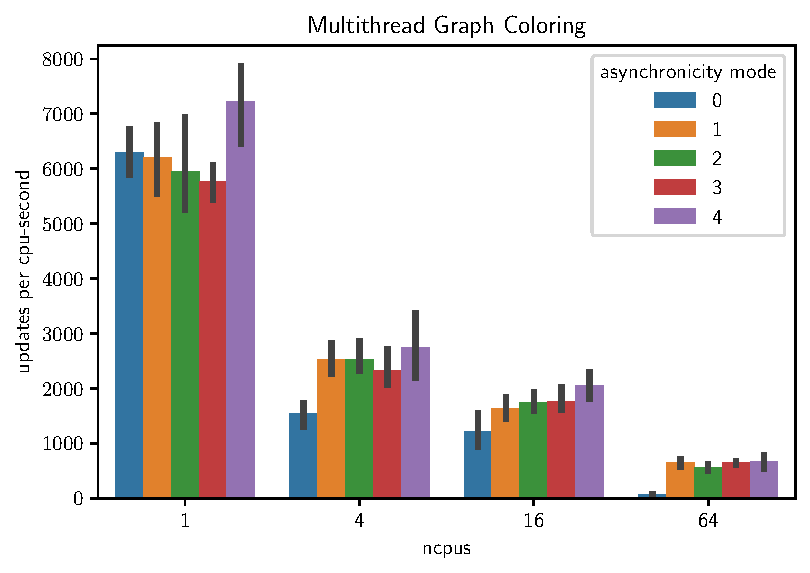
\includegraphics[width=\linewidth]{chart/multithread-graph-coloring}
     \caption{Graph coloring per-thread update rate. Higher is better.}
         \label{fig:multithread_graph_coloring_update_rate}
      \end{subfigure}
      
    \begin{subfigure}[b]{\linewidth}
      \centering
      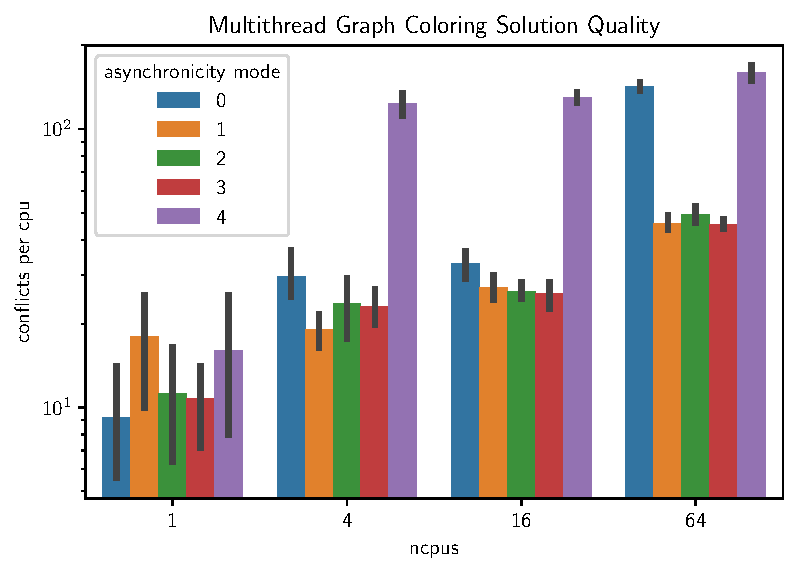
\includegraphics[width=\linewidth]{chart/multithread-graph-coloring-solution-quality}      
      \caption{Graph coloring solution conflicts. Lower is better.}
         \label{fig:multithread_graph_coloring_solution_quality}
    \end{subfigure}
    
    
    \begin{subfigure}[b]{\linewidth}
    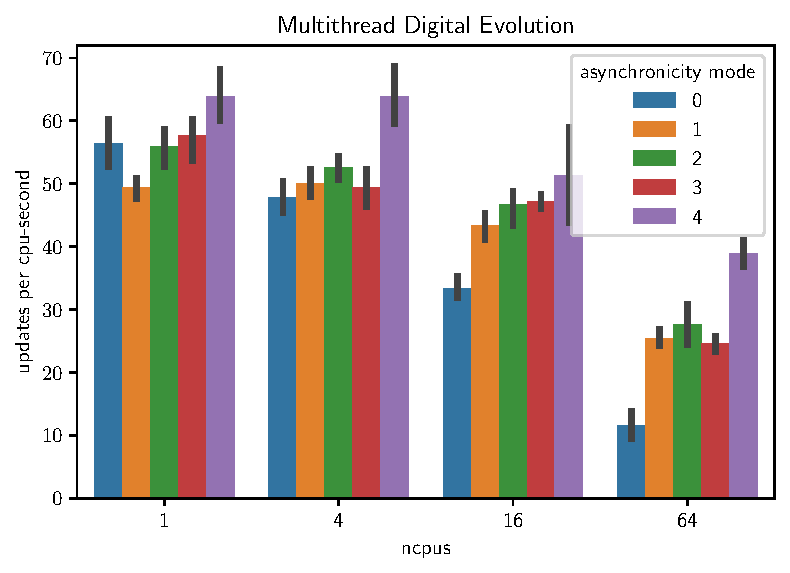
\includegraphics[width=\linewidth]{chart/multithread-digital-evolution}
    \caption{Digital evolution per-thread update rate. Higher is better.}
         \label{fig:multithread_digital_evolution_update_rate}
    \end{subfigure}

    \caption{Multithread benchmark results. Bars represent bootstrapped 95\% confidence intervals. }
      \label{fig:multithread_benchmarks}
  \end{figure}

Figure \ref{fig:multithread_graph_coloring_update_rate} presents per-cpu algorithm update rate for the graph coloring benchmark at 1, 4, 16, and 64 threads.
Update rate performance decreased with increasing multithreading across all asynchronicity modes.
This performance degradation was rather severe --- per-cpu update rate decreased by 61\% between 1 and 4 threads and by about another 75\% between 4 and 64 threads.
Surprisingly, this issue appears largely unrelated to inter-thread communication, as it was also observed in asynchronicity mode 4, where all interthread communication is disabled.
Perhaps per-cpu update rate degradation under threading was induced by strain on a limited system resource like memory cache or access to the system clock (which was used to control run timing).
This unexpectedly severe phenomenon merits further investigation to fully in future work with this benchmark.

Nevertheless, we were able to observe significantly better performance of best-effort asynchronicity modes 1, 2, and 3 at high thread counts.
At 64 threads, these run modes significantly outperformed the fully-synchronized mode 0 ($p < 0.05$, non-overlapping 95\% confidence intervals).
Likewise, as shown in Figure \ref{fig:multithread_graph_coloring_solution_quality}, best-effort asynchronicity modes were able to deliver significantly better graph coloring solutions within the allotted compute time than the fully-synchronized mode 0 ($p < 0.05$, non-overlapping 95\% confidence intervals).

Figure \ref{fig:multithread_digital_evolution_update_rate} shows per-cpu algorithm update rate for the digital evolution benchmark at 1, 4, 16, and 64 threads.
Similarly to the graph coloring benchmark, update rate performance decreased with increasing multithreading across all asynchronicity modes --- including mode 4, which eschews inter-thread communication.
Even without communication between threads, with 64 threads each thread performed updates at only 61\% the rate of a lone thread.
At 64 threads, best-effort asynchronicity modes 1, 2, and 3 exhibit about 43\% the update-rate performance of a lone thread.
Although best-effort inter-thread communication only exhibits half the update-rate performance of completely decoupled execution at 64 threads, this update-rate performance is roughly $2.1\times$ that of the fully-synchronous mode 0.
Indeed, best-effort modes significantly outperform the fully-synchronous mode on the digital evolution benchmark at both 16 and 64 threads ($p < 0.05$, non-overlapping 95\% confidence intervals).
